\section{Contraceptive Method Choice}
\label{db:sec:ds1}
\subsection{Description}
Contraceptive Method Choice contains the results of a survey. The samples are married women who were either not pregnant or do not know if they were at the time of interview. The problem is to predict the current contraceptive method choice (no use, long-term methods, or short-term methods) of a woman based on her demographic and socio-economic characteristics. The dataset has $9$ attributes and $1473$ samples. The dataset has no missing value. As it's mentioned, it has three classes. Different type of attributes such as binary, numerical and categorical as well as shortage of data make the dataset distinct and interesting for Machine Learning experiences.

\subsection{Preprocessing}
The dataset is split into three parts: $i$ Training dataset ($60\%$), $ii$ Cross Validation dataset ($20\%$) and $iii$ Test dataset ($20\%$). As it's mentioned before, shuffling algorithms of Scikit-Learn is used for splitting the dataset.

In order to scale the data, we choose Zero Mean, Min Max and 1-N vector for encoding categorical data. In order to have a better overview of result of preprocessing, we use Principal Component Analysis (PCA). By using PCA algorithm provided by Scikit-Learn, we reduce dimension of data to two and draw plots by applying different techniques. 

As it is depicted in Figure \ref{fig:db1-dimred}, the second plot seems too dense and unclear (as applying Zero-Mean on binary features may not be a good approach). By comparing the first and third plots, we can say that they seem very similar. Therefore, we use the first and the forth preprocessing method for the rest of the current section. By convention we call the first method (Numerical : Zero-Mean, Categorical : 1-N, Binary : None) $PreProc1$ and the second (Numerical : Min-Max, Categorical : 1-N, Binary : None) $PreProc2$. 

\begin{figure}
	\center
	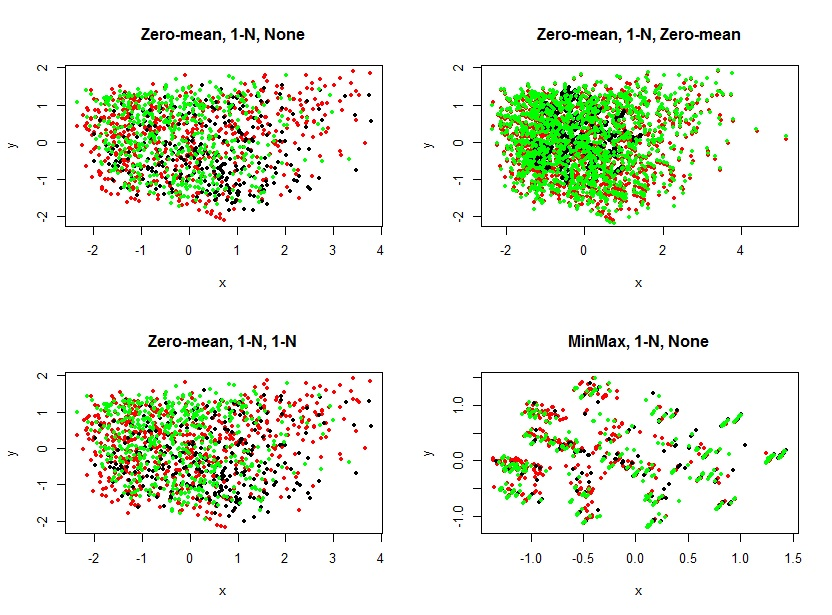
\includegraphics[scale=\figurescaling]{figures/db1/dim_reduction.jpg}
	\caption{Dimensional Reduction applied on different preprocessing techniques (Numerical, Categorical, Binary)
	\label{fig:db1-dimred}}
\end{figure}


\subsection{Logistic Regression}

\subsection{Decision Tree}

\subsection{$k$-nearest neighbor}

\subsection{Support Vector Machine}

\subsection{Neural Networks}

\subsection{Comparison}
